\documentclass[aspectratio=1610]{beamer}
% \usetheme{AnnArbor}
\usetheme{Berlin}
% \usetheme{Marburg}
% \usetheme{Malmoe}
% \usetheme{Antibes}
\usecolortheme{wolverine}
\useoutertheme{umbcfootline}
\usefonttheme{structuresmallcapsserif}
\useoutertheme{infolines}
\setbeamertemplate{headline}[Berlin]
\setbeamertemplate{navigation symbols}{Computer Security\hspace{.2cm}\includegraphics[width=1cm]{tetrophon.pdf}}
\mode<beamer>{\setbeamertemplate{blocks}[rounded][shadow=false]}
\usefonttheme[onlymath]{serif}
\date[October 2015]{October 27, 2015}
\author[H. Li, M. Kuo, A. Wong, K. Lim]{Henry Li, Matthew Kuo, Anson Wong, Kevin Lim}
\institute[UBC]{University of British Columbia\\[\medskipamount]
	% \centering
    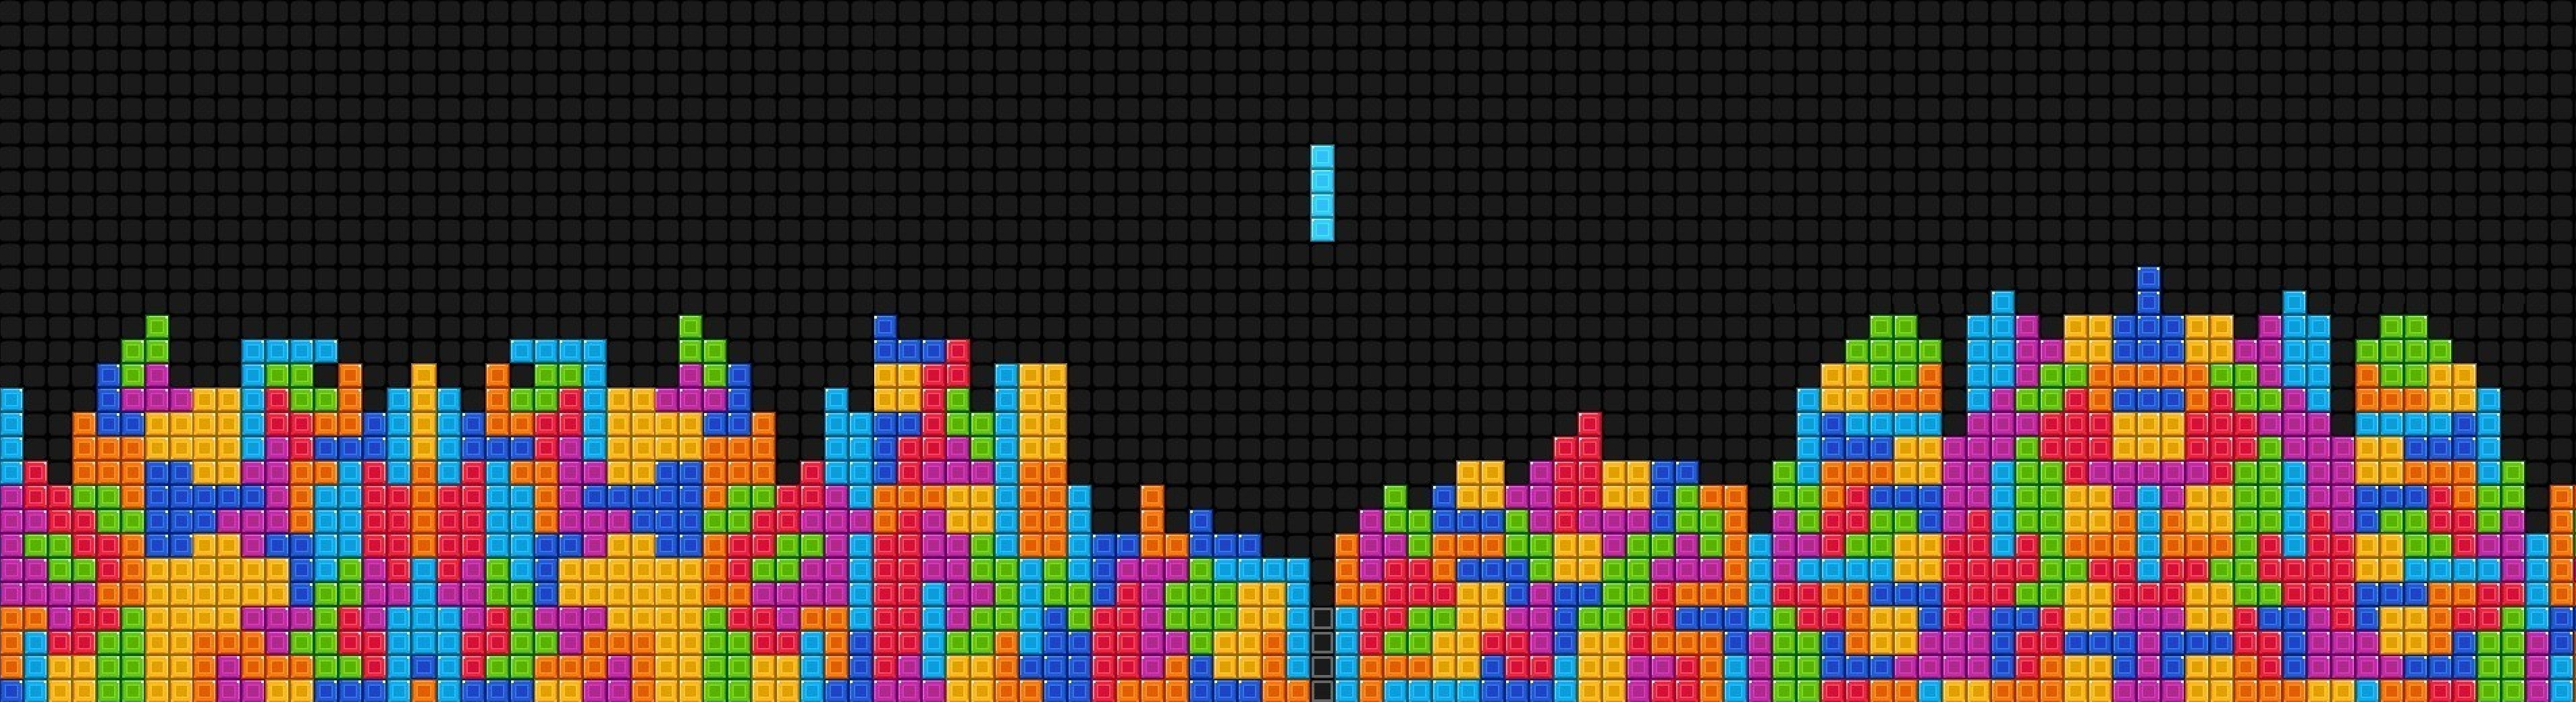
\includegraphics[height=.35\textheight]{tetrisback.png}
    }


% \institute{Foo Research Institution%}
% \title{Context-Based Surface Completion\\[\medskipamount]\centering\includegraphics[height=.2\textheight]{frontImage.pdf}}
\title[Generation T]{Generation T -- The Gamification of Password Generation}
% \subtitle{With a Discussion of Resampling Methods}

\newcommand{\tab}{\hspace*{1.5em}}

\usepackage{graphicx}
\usepackage{multicol}
\usepackage{hyperref}
% \usepackage{multimedia}
\usepackage{tikz}
\usepackage{textcomp}
\usepackage{url}

% Definition of circles
\def\firstcircle{(0,0) circle (1cm)}
\def\secondcircle{(0:1.5cm) circle (1cm)}

\colorlet{circle edge}{blue!50}
\colorlet{circle area}{blue!20}

\tikzset{filled/.style={fill=circle area, draw=circle edge, thick},outline/.style={draw=circle edge, thick}}


\begin{document}
\begin{frame}
	\titlepage
	% 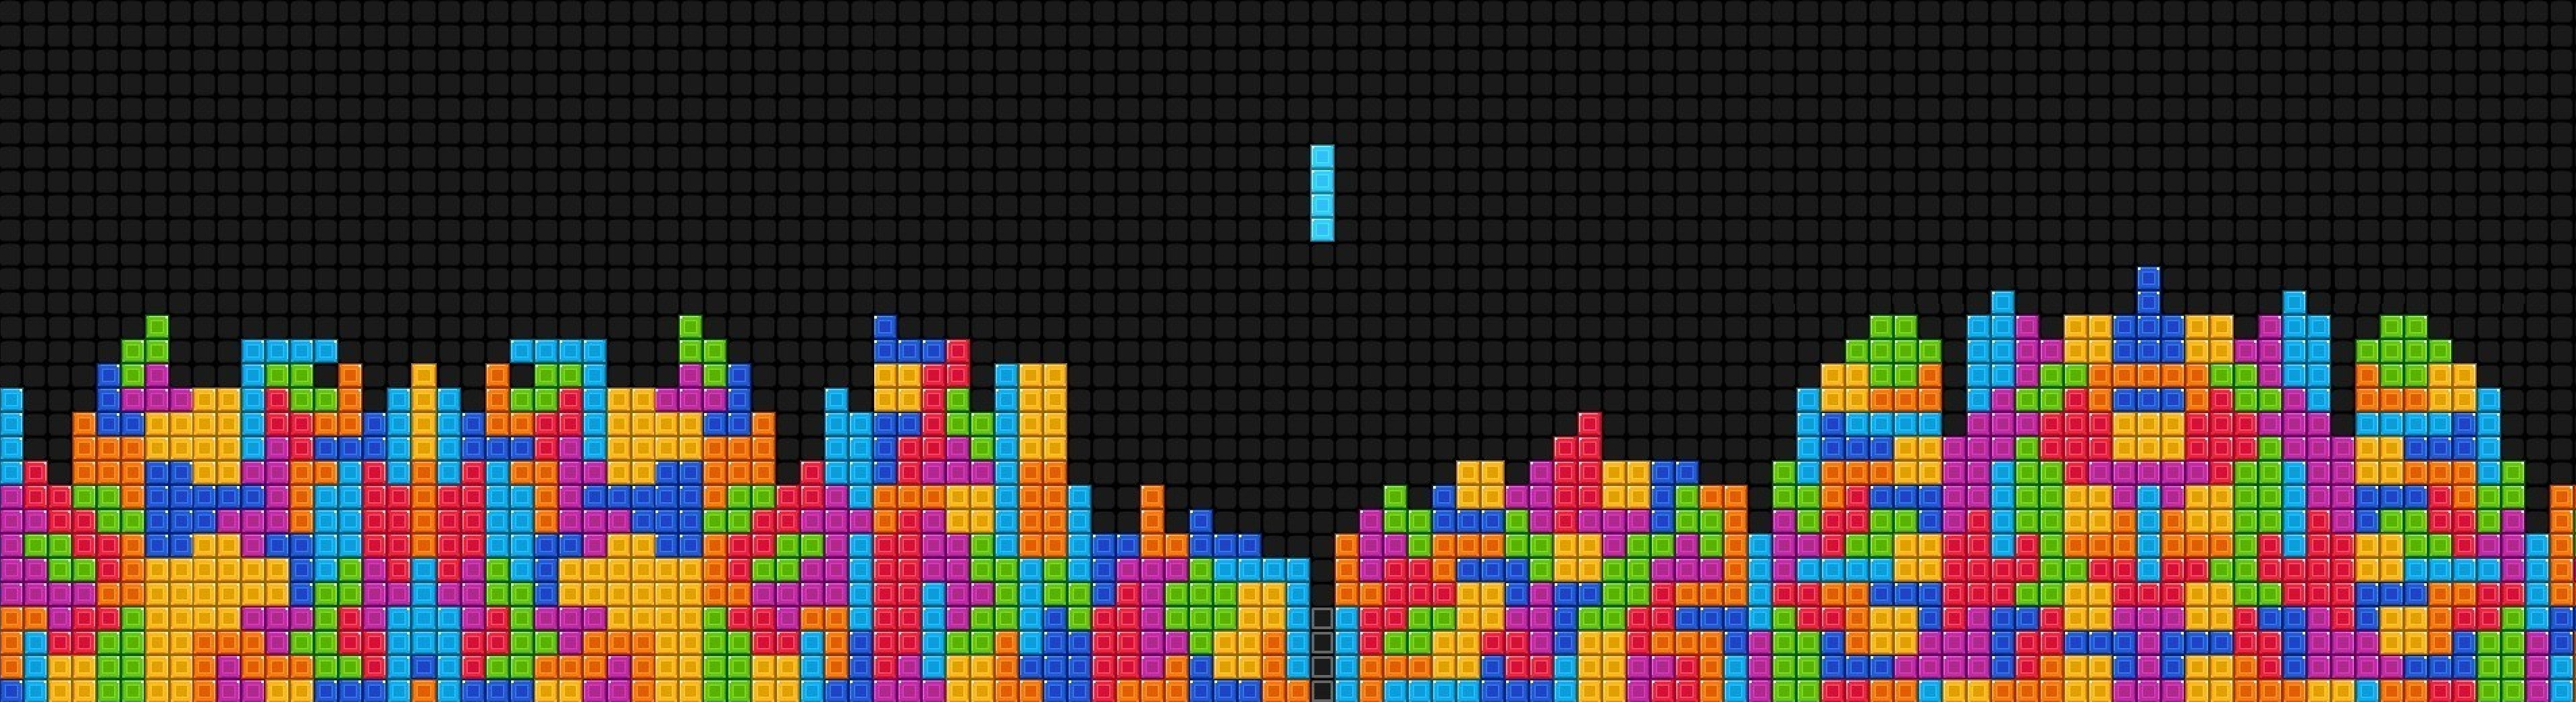
\includegraphics[height=2cm]{tetrisback.png}
\end{frame}
\begin{frame}{Introduction}
	The usual problems...
	\begin{itemize}
		\item Users do not in general choose good passwords
		\item Memorability of passwords is still a pervasive problem
		\item Memorable passwords become predictable
	\end{itemize}
	The use of \emph{gamification}
	\begin{itemize}
		\item Entice users to perform important task seen as secondary 
		\item leverage a specially designed \emph{enjoyable} task
	\end{itemize}
\end{frame}
\begin{frame}{Use Case}
	Password managers already respected as good solution.
	\begin{itemize}
		\item We do not propose to replace these solutions
		\begin{itemize}
			\item unique passwords per account is still recommended
			\item untenable to expect users to memorize unique passwords for every account (usability issue)
		\end{itemize}
		\item Complement managers
		\begin{itemize}
			\item Password managers still need to be authenticated
			\item We want a secure yet memorable password to fit this use
		\end{itemize}
	\end{itemize}
\end{frame}
\begin{frame}{Related Work}
	\begin{itemize}
		\item Shing-hon Lau, Stephen Siena, Ashutosh Pandey, Sroaj Sosothikul, Lorrie Cranor, Blase Ur and Richard Shay. \textbf{Exploring the Usability of Pronounceable Passwords.}

		\begin{itemize}
			\item 
		Lead us to the idea of using phonemes as \emph{atomic} pieces with which to construct passwords. They present some sets of useful phonemes and compares them to alphanumeric character sets. 
		\end{itemize}
		\item Sundararaman Jeyaraman and Umut Topkara. \textbf{Have the cake and eat it too -- Infusing usability into text-password based authentication systems.}

		\begin{itemize}
			\item 
		Gives a study on the use of mnemonics techniques in password generation
		\end{itemize}
		\item Andrew M. White, Fabian Monrose, Katherine Shaw and Elliott Moreton. \textbf{Isn’t that Fantabulous: Security, Linguistic and Usability Challenges of Pronounceable Tokens.}

		\begin{itemize}
			\item 
		Presents some heuristics and ratings for pronouncability of \emph{word-like strings}
		\end{itemize}
	\end{itemize}
\end{frame}
\begin{frame}{Proposed Approach}
	\begin{itemize}
		\item Use tetris to test hypothesis
		\item Put phonemes (distinct units of sound) on blocks since they lead to prounounceable passwords---more memorable (ref related works)
		\item Cleared lines construct strings to be potentially used as passwords
		\item Hopefully see if user's interaction in password generation will affect memorability of password
	\end{itemize}
	\centering
	\includegraphics[height=.5\textheight]{tetrophon.pdf}
\end{frame}
\begin{frame}{Evaluation of Our Method}
\begin{multicols}{2}	
	A-B Testing
	\begin{itemize}
		\item One group will be aware of the phonemes represented as blocks
		\item Second group will not have transparent blocks
		\item Both groups will be subject to memorization of fully automated random generation of phoneme based passwords
	\end{itemize}
	\vspace{2cm}
	\[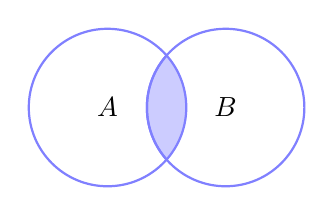
\begin{tikzpicture}
    \begin{scope}
        \clip \firstcircle;
        \fill[filled] \secondcircle;
    \end{scope}
    \draw[outline] \firstcircle node {$A$};
    \draw[outline] \secondcircle node {$B$};
\end{tikzpicture}\]
\begin{itemize}
	\item Password entry will be timed to evaluate usability of the generated passwords
\end{itemize}
\end{multicols}

Users will be invited for follow up evaluations to test password recall.
\end{frame}
\begin{frame}{Brief Security Analysis}
	Empirical study on security of passwords generated
	\begin{itemize}
		\item Will use a GPU to try and crack collected passwords
		\item We choose a representative hash function
		\item Gives a realistic strength metric given an offline scenario
	\end{itemize}
\end{frame}
\begin{frame}{Timeline}
	\begin{itemize}
		\item Prototype (\url{~}2 weeks)
		\item Conduct experiment and analysis (\url{~}1-2 weeks)
		\item Prepare film, final report and presentation (\url{~}1 week)
	\end{itemize}
\end{frame}
\begin{frame}{Conclusion}
	\begin{itemize}
		\item We explore the correlation between memorability and interaction in the generation of prounounceable passwords
		\item Limited time and scope 
		\item Invite further study on tasks focussing on interaction and memorability
	\end{itemize}
\end{frame}
\end{document}


